%!TEX root = ../dynamics.tex
\section{Predicting the Platform Throughput}\label{sec:throughput}
\begin{itemize}

	\item ML tasks: classification and regression

	\item ML results: accuracy and error

	\item Best features

\end{itemize}


% DED: push this in an appendix ..

% Feature ranking:
% ('1. feature 19 (0.650847)', 'prev')
% ('2. feature 3 (0.177595)', 'requester_id')
% ('3. feature 13 (0.062621)', 'ageminutes')
% ('4. feature 14 (0.053523)', 'leftminutes')
% ('5. feature 11 (0.037016)', 'titlelength')
% ('6. feature 12 (0.004375)', 'desclength')
% ('7. feature 0 (0.004106)', 'time')
% ('8. feature 15 (0.003591)', 'time_alloted')
% ('9. feature 1 (0.002787)', 'hour')
% ('10. feature 18 (0.002238)', 'reward')
% ('11. feature 7 (0.000434)', 'master')
% ('12. feature 8 (0.000228)', 'qualification')
% ('13. feature 5 (0.000188)', 'totalapproved')
% ('14. feature 17 (0.000160)', 'totalhis')
% ('15. feature 16 (0.000159)', 'totalbatchs')
% ('16. feature 4 (0.000128)', 'location')
% ('17. feature 9 (0.000003)', 'bonus')
% ('18. feature 10 (0.000001)', 'invite')
% ('19. feature 6 (0.000000)', 'approvalrate')
% ('20. feature 2 (0.000000)', 'weekday')




\begin{figure}[htbp]
	\centering
		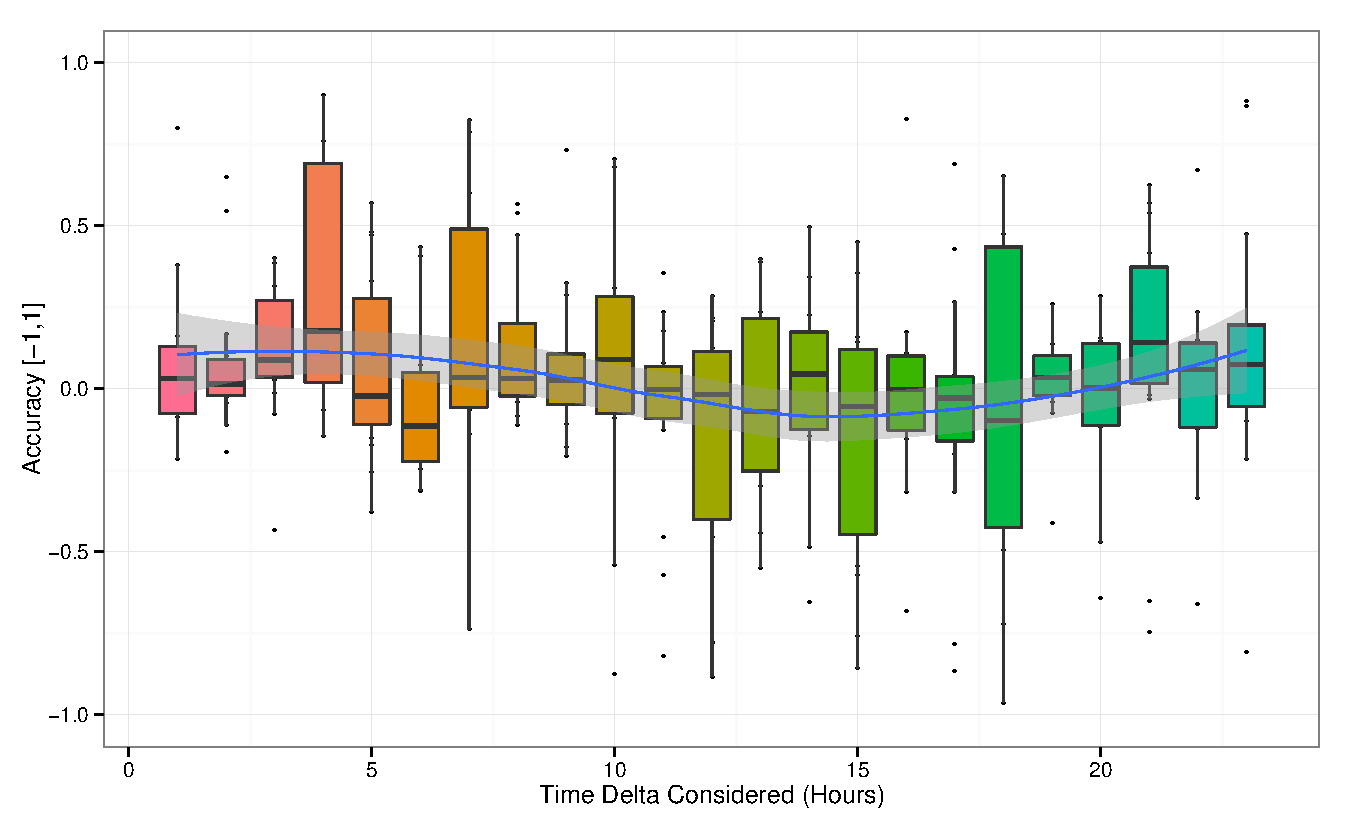
\includegraphics[width=0.5\textwidth]{figures/ML_accuracy}
	\caption{Accuracy of the throughput prediction when considering larger training sets for the prediction.}
	\label{fig:accuracy}
\end{figure}

\begin{figure}[htbp]
	\centering
		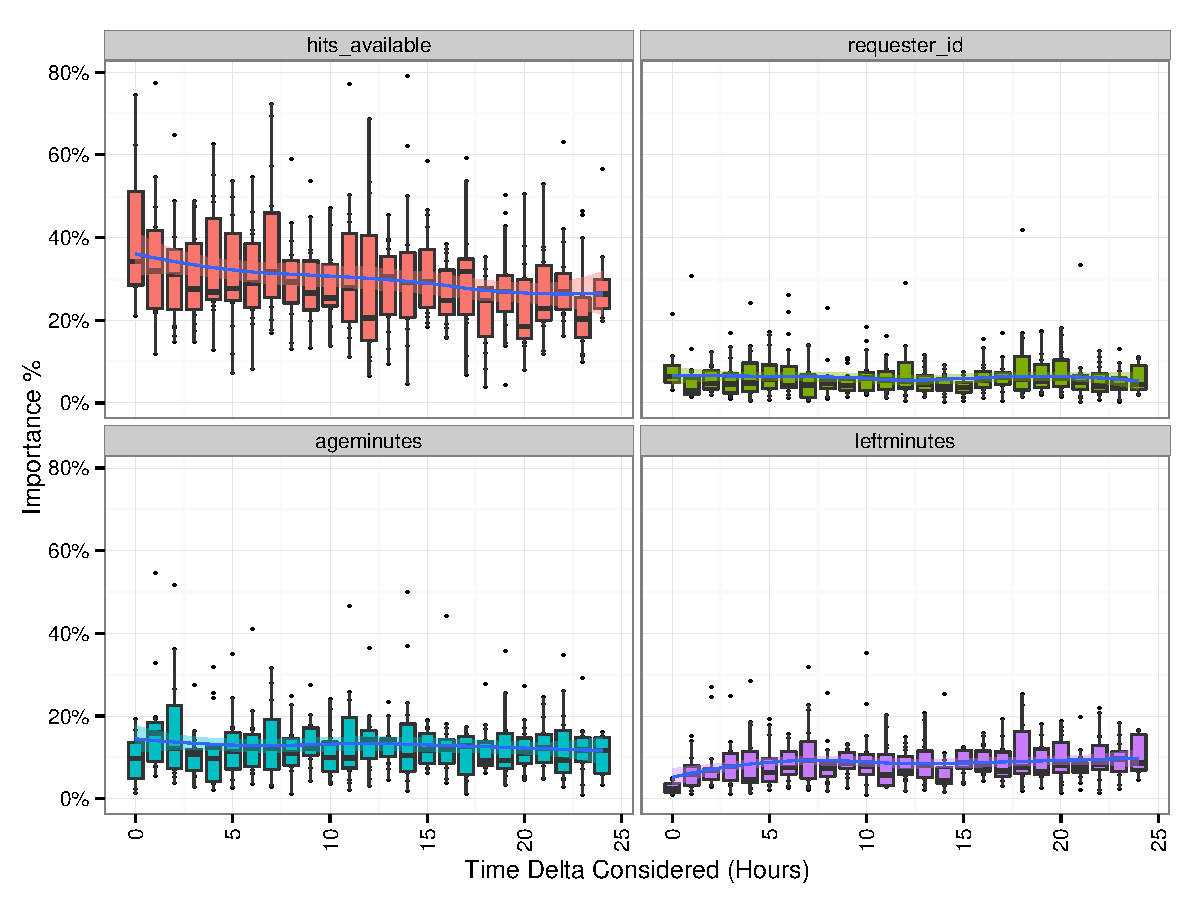
\includegraphics[width=0.5\textwidth]{figures/importances}
	\caption{Feature importance when considering larger training sets for the prediction.}
	\label{fig:falsepred}
\end{figure}
